\section{Calcul parallèle}

\subsection{}

\begin{quotation}
  1. Quelles caractéristiques le rendent difficile à paralléliser ?
\end{quotation}

Le calcul aux différentes profondeurs n'est pas parallélisable,
puisque la valeur d'un pixel à la profondeur $n+1$ est une fonction
complexe de la valeur de ce pixel à la profondeur $n$. De plus, telle
que la fonction est codée, la valeur à la profondeur $n+1$ écrase en
mémoire celle à la profondeur $n$.

En revanche, si l'on excepte l'expression de $x$ et de $y$, chaque
pixel de l'image subit le même traitement, qui ne dépend pas de la
valeur d'autres pixels. Cette portion de code pourrait donc être
parallélisable.

En l'état, la mise à jour des variables $x$ et $y$ est fonction de
leur valeur antérieure.  Néanmoins, ces variables sont des suites
arithmétiques, et peuvent donc être calculées de manière explicite :

\[ \begin{cases}
    x_n = x_{n-1} + x_{incr}\\
    y_n = y_{n-1} + y_{incr}
  \end{cases} \]

\[\textrm{donne :} \begin{cases}
    x_{i w + j} = x_{min} + j \times x_{incr}\\
    y_{i w + j} = y_{min} + i \times y_{incr}
  \end{cases} \]


\begin{quotation}
  2. Proposer plusieurs stratégies pour paralléliser le code
  séquentiel en détaillant les choix techniques à prendre.

  3. Donner les algorithmes de chacunes de vos stratégies de
  parallélisation.

  4. [...] adapter à une architecture parallèle à mémoire distribuée
  exploitée au moyen de MPI.
\end{quotation}

\subsubsection{Équilibrage statique}

Une première approche est de partager uniformément les blocs d'image à
calculer entre les processus. Puisque notre image est stockée
linéairement, il sera plus facile de traiter des lignes
entières. Ainsi, pour une image de hauteur $h$ lignes, chacun des $p$
processus aura à traiter $h_{local} = h / p$\footnote{Dans le code,
  pour éviter des confusions entre $h_{local}$ (hauteur) et
  $h_{local} \times w$ (indice), on a défini $nlines = h / p$.}
lignes. Il faut alors vérifier que $p$ divise $h$, afin d'obtenir un
nombre entier de lignes : cela simplifie l'algorithme et évite les
erreurs d'arrondi.

Plus précisément, le $r$\ieme processus, $r \in \{0, \ldots, p-1\}$,
devra traiter les lignes
$[ r \times h_{local}, (r+1) \times h_{local} -1 ]$. Tout cela se
résume à la figure \ref{fig:mandel:decoupage-statique}.

\begin{figure}[h]
  \centering

  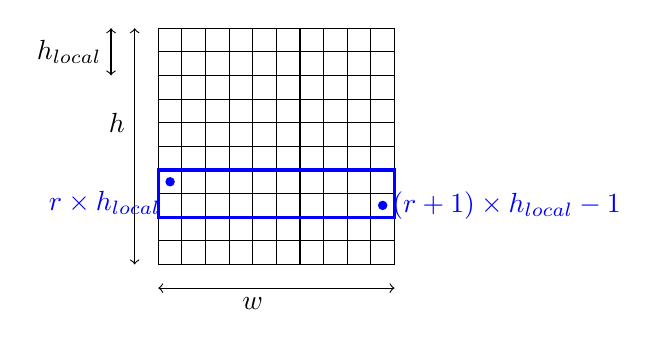
\begin{tikzpicture}[scale=0.3]
    % Colonnes
    \foreach \x in {-5, ..., 5} {
      \draw[thin] (\x, -5) -- (\x, 5);
    }
    % Lignes
    \foreach \y in {-5, ..., 5} {
      \draw[thin] (-5, \y) -- (5, \y);
    }

    % Dimensions
    \draw[<->] (-6, -5) -- (-6, 5) node[left, pos=0.6] {$h$};
    \draw[<->] (-5, -6) -- (5, -6) node[below, pos=0.4] {$w$};
    \draw[<->] (-7, 3) -- (-7, 5) node[left, pos=0.5] {$h_{local}$};

    % Premier et derniers pixels
    \draw[very thick, blue] (-5,-1) -- (5,-1) -- (5,-3) -- (-5,-3) -- cycle;
    \fill[blue] (-4.5, -1.5) circle [radius=0.2] node[blue, below left]
    {$r \times h_{local}$};
    \fill[blue] (4.5, -2.5) circle [radius=0.2] node[blue, right]
    {$(r+1) \times h_{local}-1$};
  \end{tikzpicture}

  \caption{Découpage statique de l'i\-ma\-ge (processus \no 4 sur 5)}
  \label{fig:mandel:decoupage-statique}
\end{figure}

Puisque chaque processus connaît la partie de l'image qu'il doit
traiter, il n'y a besoin d'aucune communication entre les processus
avant le début du calcul. En ce qui concerne l'assemblage des blocs de
l'image calculés, le comportement varie en fonction de l'organisation
de la mémoire. Pour une architecture à mémoire partagée, puisque
chaque processus accède à une zone de mémoire qui lui est propre, il
n'y a aucune précaution à prendre. Pour une architecture à mémoire
distribuée, chaque processus devra envoyer son bloc d'image
(\texttt{MPI\_Gather})\footnote{Le code correspondant étant pédagogique,
  il utilise un Send/Receive, plus facile}. C'est le but de
l'algorithme \ref{alg:mandel:stat:envoi}.

\begin{algorithm}
  \caption{Allocation de la mémoire}
  \label{alg:mandel:stat:memoire}
  \Donnees{\;
    \begin{tabular}{l @{ : } l}
      \H & hauteur totale de l'image\\
      \W & largeur totale de l'image\\
      \Rank & rang du processus (connu)\\
      \Hlocal & hauteur d'un bloc (calculé)
    \end{tabular}
  }

  \Res{\;
    \begin{tabular}{l @{ : } l}
      \Ima & pointeur vers le début de l'image\\
      \Pima & pointeur vers le pixel courant
    \end{tabular}
  }

  \Deb{%
    \uSi{\Rank == \MASTER}{%
      \hangindent=\skiptext\hangafter=1
      \Pima = \Ima = \malloc{\H * \W * \sizeof{unsigned char}}\;
    }
    \Sinon{%
      \hangindent=\skiptext\hangafter=1
      \Pima = \Ima = \malloc{\Hlocal * \W * \sizeof{unsigned char}}\;
    }
    Test de l'allocation\;
  }
\end{algorithm}

\begin{algorithm}
  \caption{Calcul des pixels}
  \label{alg:mandel:stat:pixels}
  \Donnees{\;
    \W, \Rank, \Hlocal, \Pima

    \begin{tabular}{l @{ : } l}
      \Xmin, \Ymin & coords complexes min.\\
      \Xincr, \Yincr & incrément des coords
    \end{tabular}
  }
  \Variables{\;
    \begin{tabular}{l @{ : } l}
      $x, y$ & coordonnées courantes\\
      $i, j$ & ligne, colonne courante\\
    \end{tabular}
  }

  \Deb{%
    $y$ = \Ymin + \Yincr * \Rank * \Hlocal\;
    \Pour{$i$ de 0 à \Hlocal}{%
      \tcp{Idem algo séquentiel}
    }
  }
\end{algorithm}

\begin{algorithm*}
  \caption{Envoi / réception des blocs}
  \label{alg:mandel:stat:envoi}
  \Donnees{\W, \Rank, \Hlocal, \Ima, \Pima}
  \Variables{\;
    \begin{tabular}{l @{ : } l}
      $s$ & processus source\\
      $status$ & infos sur le message
    \end{tabular}
  }

  \Deb{%
    \uSi{\Rank == \MASTER}{%
      \PourTous{esclaves}{%
        \tcp{Attente d'un message}
        \Probe{\AnySource, 0, \CommWorld, \textsf{\&}$status$}\;
        $s$ = $status$.\Source\;
        \Si{$s$ != \MASTER}{%
          \tcp{Assemblage du bloc}
          \hangindent=\skiptext\hangafter=1
          \Recv{\Ima~+~$s$~*~\W~*~\Hlocal~*~\sizeof{unsigned~char},
            \Hlocal~*~\W, \Char, $s$, 0, \CommWorld,
            \textsf{\&}$status$}\;
        }
      }
      Sauvegarde de l'image\;
      Affichage du chronomètre\;
    }
    \Sinon{%
      \hangindent=\skiptext\hangafter=1
      \Send{\Ima, \W~*~\Hlocal, \Char, \MASTER, 0, \CommWorld}\;
    }
  }
\end{algorithm*}


\subsubsection{Équilibrage dynamique}

Bien que ce ne soit pas le cas ici, puisque le coût de
\texttt{xy2color} ne dépend pas des valeurs de $a$ ou de $b$, il
existe des situations où toutes les zones de l'image n'ont pas le même
coût de traitement. Pour s'entraîner, nous allons appliquer ici un
algorithme à répartition dynamique des charges.

Dans les algorithmes \ref{alg:mandel:dyn:maitre} et
\ref{alg:mandel:dyn:esclave}, une approche maître--esclave est mise en
place. Un maître, de rang 0\footnote{Ce n'est qu'une convention, le
  rang du processus maître pourrait avoir toute valeur comprise dans
  $\{0, \ldots, p-1\}$, tant que tous les processus ont la même
  (paramètre en ligne de commande).}, a pour tâche de recevoir les
lignes traitées par les esclaves et, si besoin, de leur envoyer
d'autres lignes à traiter. Il ne participe pas au traitement.

Comme précédemment, au lancement du programme, tous les esclaves
disposent de l'intégralité des informations dont ils ont besoin pour
lancer le calcul. Le nombre de blocs est alors un argument du
programme.

Cet algorithme est caractérisé par sa \emph{granularité}, qui est le
nombre de lignes dans chaque tâche élémentaire.

\SetKwData{Result}{RESULT\_BLOC}
\SetKwData{Data}{RESULT\_DATA}
\SetKwData{Work}{WORK}
\SetKwData{Nblocks}{nblocks}

\begin{algorithm*}
  \caption{Gestion des processus esclaves en charge dynamique
    (\emph{maître})}
  \label{alg:mandel:dyn:maitre}

  \Donnees{\W, \Hlocal, \Ima\;

    \begin{tabular}{l @{ : } l}
      \Nblocks & nombre de blocs (calculé)
    \end{tabular}
  }

  \Variables{$s$, $status$\;
    \begin{tabular}{l @{ : } l}
      $current\_block$ & indice du bloc à envoyer\\
      $block$ & indice du bloc reçu
    \end{tabular}
  }

  \Deb{%
    \Pour{$current\_block$ de \P-1 à (\Nblocks + \P -1)}{
      \hangindent=\skiptext\hangafter=1
      \tcp{1. Réception du numéro de bloc achevé}
      \Probe{\AnySource, \Result, \CommWorld, \textsf{\&}$status$}\;
      $s$ = $status$.\Source\;
      \Recv{\textsf{\&}$block$, 1, \Int, $s$, \Result, \CommWorld,
        \textsf{\&}$status$}\;

      \tcp{2. Réception des données}
      \hangindent=\skiptext\hangafter=1
      \Recv{\Ima~+~\W~*~\Hlocal~*~$block$~*~\sizeof{unsigned~char},
        \Hlocal~*~\W, \Char, \Data, \CommWorld, \textsf{\&}$status$}\;

      \tcp{3. Envoi d'un nouveau bloc}
      \hangindent=\skiptext\hangafter=1
      \nlset{$\triangleright$}\Send{\textsf{\&}$current\_block$,
        1, \Int, $s$, \Work, \CommWorld}\;\label{ligne}
    }
    Sauvegarde de l'image\;
  }
\end{algorithm*}

L'algorithme du processus maître ainsi modélisé autorise le maître à
envoyer un numéro de bloc potentiellement invalide car trop élevé
(ligne \ref{ligne}).

\begin{algorithm*}
  \caption{Calcul en charge dynamique (\emph{esclave})}
  \label{alg:mandel:dyn:esclave}

  \Donnees{\W, \Hlocal, \Ima, \Nblocks, \Xmin, \Ymin, \Xincr, \Yincr}

  \Variables{$y$, $s$, $status$, $block$}

  \Tq(\tcp*[h]{$block$ est valide}){$block < $ \Nblocks}{
    \tcp{Travail : idem algorithme \ref{alg:mandel:stat:pixels} avec :}
    $y$ = \Ymin + \Yincr * $block$ * \Hlocal\;

    \tcp{Envoi du résultat}
    \hangindent=\skiptext\hangafter=1
    \Send{\textsf{\&}$block$, 1, \Int, \MASTER, \Result, \CommWorld}\;
    \hangindent=\skiptext\hangafter=1
    \Send{\Ima, \W * \Hlocal, \Char, \MASTER, \Data, \CommWorld}\;

    \tcp{Réception de travail}
    \hangindent=\skiptext\hangafter=1
    \Recv{\textsf{\&}$block$, 1, \Int, \MASTER, \Work, \CommWorld, 
      \textsf{\&}$status$}\;
  }
\end{algorithm*}

%%% Local Variables:
%%% mode: latex
%%% TeX-master: "../rapport"
%%% End:
